In this section, we will look at the foundations of the analyzed tools, Proverif and Tamarin prover.


\section{Proverif}
Let us start with a brief overview of Proverif internal reasoning. For more information, please refer to \cite{SymbolicComputationalBlanchet, SymbolicVerificationBlanchet, ProverifManual}.

\subsection{High level view}
Proverif protocol specification is based on an extended version of the \pic{} (the \textit{applied} \pic{}). The tool also allows the user to define constructors, destructors and equations\footnote{Destructors are basically used to de-construct some previously constructed term (e.g. decryption of an encrypted ciphertext), while equations represent term equality of some sort (e.g. commutativity of multiplication).}, which form the cryptographic primitives. Security properties are modeled using \Horncs{}. The entire protocol is then automatically translated to a set of \Horncs{}. Using this abstract representation of the protocol, the Proverif verifier uses a resolution algorithm on such clauses that allow for verification of security properties \cite{SymbolicComputationalBlanchet}.
A graphical representation of the process is given in \cref{fig:proverif-verification-method}.

It is important to note that Proverif is not complete. We will consider implications in \cref{sec:comparison}. Moreover, it may not terminate, but it has been proven to be precise and efficient enough in practice by many case studies (the following is a non-exhaustive list of examples \cite{10.1145/1266977.1266978, ABADI20053, MTProto2-Proverif, hal-01575923}).
We will now proceed with an overview of \pic{} and \Horncs{}.

\begin{figure}[t]
    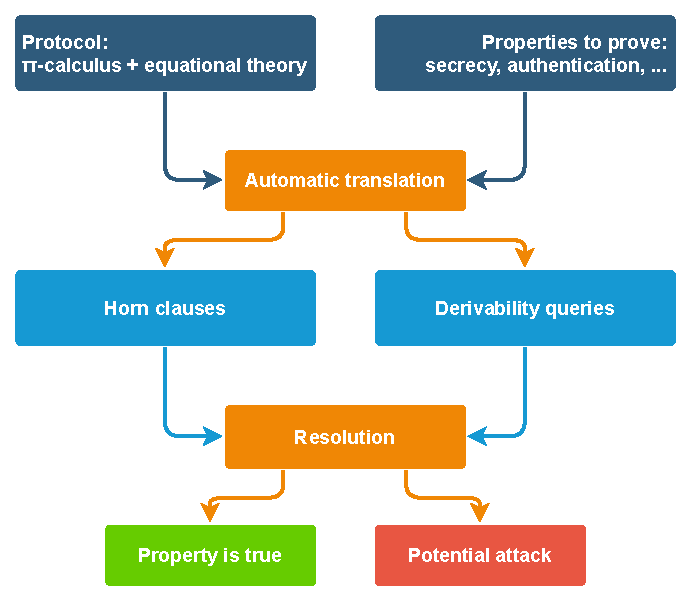
\includegraphics{proverif-verification-method}
    \centering
    \caption{Proverif verification method.\\Inspired by a representation from \BLANC{} \cite{SymbolicComputationalBlanchet}.}
    \label{fig:proverif-verification-method}
\end{figure}

\subsection{\pic{} and \apic{}}
\label{subsec:pic-apic}

The \pic{} \cite{pi-calculus-book} is a (minimal) programming language that models a system communicating on channels. It belongs to the \textit{process calculi} family, which is generally used to model concurrent systems. As Proverif uses the \textit{applied} \pic{} (which is an extension of standard \pic{}{}), we will briefly present its syntax in the rest of this section.

The following description of \apic{} references articles \cite{applied-pi-calculus-abadi-1, applied-pi-calculus-abadi-2, applied-pi-calculus-private-auth}. Please refer to these resources for further information and a more formal or in-depth description. For brevity, we only define the main features of \apic{} in \cref{subsub:syntax-apic}.

\paragraph{Overview of the syntax of the \apic{}}
\label{subsub:syntax-apic}

A \textit{signature \textSigma} is composed by a finite number of functions symbols, each with its own integer arity. Given such signature, together with an infinite set of names and an infinite set of variables, the set of \textbf{terms} is defined by the grammar:

\begin{equation}
    \label{eq:apic-terms}
    \begin{aligned}
        U, V & ::=                        \\
             & a, b, \ldots               \\
             & x, y, \ldots               \\
             & \func{f}{U_1, \ldots, U_l}
    \end{aligned}
    \qquad
    \begin{aligned}
        \mbox{term} & \mbox{s}                       \\
                    & \mbox{name}                    \\
                    & \mbox{variable}                \\
                    & \mbox{constructor application}
    \end{aligned}
\end{equation}

where $f \in \Sigma$ and $l$ matches the arity of $f$. Next, we define a grammar for processes, which is shown in \cref{eq:apic-processes}. As pointed to by Microsoft researchers, this grammar is very similar to the \pic{} \cite{applied-pi-calculus-private-auth}. We will omit to define differences from standard \pic{} as we have not formally defined \pic{} either.

\begin{equation}
    \label{eq:apic-processes}
    \begin{aligned}
        P, Q & ::=                \\
             & 0                  \\
             & \apicin{c}{x}{P}   \\
             & \apicout{c}{x}{P}  \\
             & \apicpc{P}{Q}      \\
             & \apicrep{P}        \\
             & \apicnew{vn}{P}    \\
             & \apicif{M=N}{P}{Q}
    \end{aligned}
    \qquad
    \begin{aligned}
        \mbox{proc} & \mbox{esses}                        \\
                    & \mbox{null process}                 \\
                    & \mbox{message input}                \\
                    & \mbox{message output}               \\
                    & \mbox{parallel composition}         \\
                    & \mbox{replication}                  \\
                    & \mbox{name restriction (``fresh'')} \\
                    & \mbox{conditional}
    \end{aligned}
\end{equation}

The null process $0$ does nothing;
$\apicin{c}{x}{P}$ ($\apicout{c}{x}{P}$) gets (outputs) the message $x$ from (into) channel $\overline{c}$ ($c$) and then continues with process $P$; Notice that getting a message from a channel is a blocking operation;
$\apicpc{P}{Q}$ is the parallel composition of $P$ and $Q$;
The process $\apicrep{P}$ effectively behaves as an infinite number of copies of $P$ running in parallel (\textit{unbounded} replication);
$\apicnew{vn}{P}$ creates a new fresh value, before proceeding with process $P$;
$\apicif{M}{P}{Q}$ is a standard conditional.

\subsection{\Horncs{}}

As we said earlier, Proverif's analysis is based on \Horncs{}. Let us define them.

The class of Horn formulas is obtained by restricting the form of the conjuncts in a proposition in conjunctive normal form. Consider a proposition $A$ in conjunctive normal form $C_1 \land \ldots \land C_n$, where each $C_i$ is a conjunction of either positive or negative literals. A is a \Hornc{} if and only if each $C_i$ contains at most one positive literal \cite{DOWLING1984267,horn_1951}. Additionally, every variable in a clause is implicitly universally quantified.


\subsection{Intuition for the translation to \Horncs{}}
For this section we will consider \Horncs{} in the following form: $F_1 \land \ldots \land F_n \Rightarrow F$.
Additionally, the literal $\attack{x}$ will be used to denote that the attacker knows the term $x$.

Proverif automatically translates cryptographic primitives, attacker capabilities, and the protocol itself to \Horncs{}. In the following paragraphs, we will show some translations that Proverif applies. Most of the examples are taken from \BLANC{} \cite{blanchet:hal-01110425}.

\paragraph{Representation of cryptographic primitives}
As already seen, Proverif represents cryptographic primitives as constructors and destructors. A destructors $g$ is defined as a set $\func{def}{g}$ of rewrite rules of the form $g\left(M_1, \ldots, M_n\right) \rightarrow M$, where $M_1, \ldots, M_n, M$ are terms that contain variables and constructors and the variables in $M$ all occur in $M_1, \ldots, M_n$.


\paragraph{Representation of attacker capabilities}
During its computation, the attacker can apply constructors and destructors. Let us define a constructor of arity $n$ as $\func{f}{x_1, \ldots, x_n}$. We can model it with the following clause:

\begin{equation}
    \attack{x_1} \land \ldots \land \attack{x_n} \Rightarrow \attack{\func{f}{x_1,\ldots,x_n}}
\end{equation}

This is consistent with the symbolic model: the adversary needs to know every term to apply a constructor.
Now, suppose that $g$ is a destructor. For each rewrite rule $\func{g}{M_1 \land \ldots \land M_n} \rightarrow M$ in $\func{def}{g}$ we have the following clause:

\begin{equation}
    \attack{M_1} \land \ldots \land \attack{M_n} \Rightarrow \attack{M}
\end{equation}

Notice that the destructor did not appear in the \Hornc{}, and never will. Instead, we use pattern matching to model them. For example, let us show how we can model public-key encryption:

\begin{equation}
    \begin{alignedat}{3}
        & \mbox{aenc} \qquad && \attack{m} \land \attack{pk} \Rightarrow \attack{\func{aenc}{m, pk}}            \\
        & \mbox{pk} \qquad   && \attack{sk} \Rightarrow \attack{\func{pk}{sk}}                                  \\
        & \mbox{adec} \qquad && \attack{\func{aenc}{m, \func{pk}{sk}}} \land \attack{sk} \Rightarrow \attack{m}
    \end{alignedat}
\end{equation}

The first two equation model the constructors $\func{aenc}{m, pk}$ and $\func{pk}{sk}$. The third models asymmetric decryption, defined as $\func{adec}{\func{aenc}{m, \func{pk}{sk}}, sk}$.

\sloppy We also model a revealing signing scheme, formed by two constructors $\func{sign}{m, sk}$ and $\func{pk}{sk}$ and from the rewrite rules $\func{getmess}{\func{sign}{m, sk}} \rightarrow m$ and $\func{verify}{\func{sign}{m, sk}, \func{pk}{sk}} \rightarrow m$, respectively used for message revealing and for signature verification. \Cref{eq:signing-horn-clauses} shows the representation of this primitives as \Horncs{}.

\begin{equation}
    \label{eq:signing-horn-clauses}
    \begin{alignedat}{3}
        & \mbox{sign} \qquad    && \attack{m} \land \attack{sk} \Rightarrow \attack{\func{sign}{m, sk}}            \\
        & \mbox{getmess} \qquad && \attack{\func{sign}{m, sk}} \Rightarrow \attack{m}                              \\
        & \mbox{verify} \qquad  && \attack{\func{sign}{m, sk}} \land \attack{\func{pk}{sk}} \Rightarrow \attack{m}
    \end{alignedat}
\end{equation}

\paragraph{Representation of the protocol}

Let us show how the protocol below can be written as \Horncs{}. We additionally leave the attacker the task of starting the protocol, that is, the attacker will send the public key of the responder to A.

\begin{enumerate}
    \label{enum:protocol}
    \item A $\rightarrow$ B: $\func{aenc}{\func{sign}{k, skA}, pkB}$
    \item B $\rightarrow$ A: $\func{senc}{m, k}$
\end{enumerate}

The responder of the protocol can either be B or the attacker. In both cases, we can model this with:

\begin{equation}
    \attack{\func{pk}{x}} \Rightarrow \attack{\func{aenc}{\func{sign}{k, skA}, \func{pk}{x}}}
\end{equation}

When B receives the message, he decrypts it with his secret key $skB$. Then, B tests the signature evaluating $\func{verify}{x', pkA}$, which succeeds if and only if $x' = \func{sign}{y, skA}$. If so, B sends a secret constant $m$ using the encryption key $k$. We assume that the attacker relays the message coming from A, and intercepts the message sent by B. Hence, the following clause models the second message of the protocol:

\begin{equation}
    \attack{\func{enc}{\func{sign}{y, skA}, \func{pk}{skB}}} \Rightarrow \attack{\func{senc}{m, y}}
\end{equation}






\section{Tamarin prover}
\label{sec:tamarin-foundations}
In this section, we will see an overview of Tamarin's foundations and internal reasoning.
For a more in-depth description and further information, see the Tamarin foundations paper \cite{TamarinFoundations} or the extended foundations paper \cite{TamarinFoundationsExtended}.

\subsection{High level view}
First of all, let us examine a high-level picture of Tamarin.

The security property model of Tamarin is based on labeled multiset rewriting rules to specify protocols and adversary capabilities, a guarded fragment\footnote{Only a few examples of formulas respecting the guarded fragment of first-order logic used by Tamarin will be given in \cref{sub:guarded-formulas}. See \cite{FragmentFirstOrderLogicPaper} for a rigorous definition from a mathematical point of view.} of first-order logic to specify security properties\footnote{Security properties in Tamarin will also be referred to as \textit{lemmas}.} and functions and equational theories to model the algebraic properties of cryptographic protocols \cite{TamarinFoundations}.
Finally, Tamarin uses a novel constraint-solving algorithm to validate or falsify lemmas.

In other words, Tamarin allows to specify a labeled transition system that induces a set of traces and offers automatic verification of such traces using a guarded fragment of first-order logic to specify ``good'' traces. Tamarin then tries to prove the negation of the specified ``good'' traces.

Tamarin also offers built-in equational theories \cite{TamarinProverManual}. A brief overview will be given in \cref{sub:built-in-equational-theories}.

\subsection{Terminology}
\label{subsec:tamarin-foundations-terminology}
As reported earlier, multiset rewriting rules are used to specify adversary capabilities and protocols. More precisely, a \textit{set} of \textit{labeled} multiset rewriting rules are used.

The ingredients of this multiset rewriting system are the following:

\begin{description}[style=nextline]
    \item[Terms] which can be essentially thought of as messages. Terms can be of three different sorts. The more general sort is the \textit{msg} sort, which has two incomparable sub-sorts \textit{fresh} and \textit{pub} for fresh and public names, respectively;
    \item[Facts] which model information in the protocol. Facts have an arity, can be linear or persistent and are composed by terms. Linear facts model resources that can be consumed once, while persistent facts can be consumed an arbitrary number of times (and are prefixed by an exclamation mark). By convention, facts always start with a capital letter;
    \item[Special facts] Four facts are reserved and are used to model the freshness of a message $t$ ($\mbox{\textbf{Fr}}\left(t\right)$), a message $t$ coming from the public channel ($\mbox{\textbf{In}}\left(t\right)$), a message $t$ to send to the public channel ($\mbox{\textbf{Out}}\left(t\right)$) and knowledge of a certain message $t$ from the attacker ($\mbox{\textbf{K}}\left(t\right)$);
    \item[State of the system] The state of the system is represented using a \textit{multiset} of facts;
    \item[Transition rules] A multiset of transition rules defines the possible transitions from one state to another one. Transitions are denoted with the following syntax
        \begin{equation}
            \msr{L}{A}{R}
        \end{equation}
        where $L, A$ and $R$ are multisets of facts, respectively called \textbf{premises}, \textbf{actions} and \textbf{conclusions}.
    \item[Trace] A trace is a sequence $\left<A_1, \ldots, A_n\right>$ of sets of ground facts denoting the sequence of actions that happened during a protocol's execution.
\end{description}


\subsection{Transition rules}
\label{sub:Transition-rules}
Let us examine an informal description of transitions.

\begin{itemize}
    \item{Let $S$ be the current state of the system}
    \item{Let $\msrnolabel{L}{R}$ be a transition rule. Note that this is a \textit{multiset rewriting rule} without a \textit{label};}
    \item{Let $\msrnolabel{l}{r}$ be a ground instance of the rule (i.e. no variables are found in the multisets);}
    \item{If we apply $\msrnolabel{l}{r}$ (assuming $l \msrsubseteq S$) to our state $S$ we reach a new state, defined by the following equation:
                \begin{equation}
                    S' = S \msrsetminus l \msrcup r
                \end{equation}
                We use $\msrsetminus$, $\msrcup$ and $\msrsubseteq$ to define difference, union and subset over multisets, respectively. We can also consider the difference between linear and persistent facts and define $\lin{l}$ ($\pers{l}$) as linear facts (persistent facts) in $l$. Assuming that $\lin{l} \msrsubseteq S$ and $\pers{l} \msrsubseteq S$, then the equation becomes the following:
                \begin{equation}
                    S' = S \msrsetminus \lin{l} \msrcup r
                \end{equation}
                It should be clear from the equation why persistent facts can be consumed any number of times: they are never removed from the state of the system. This can be useful in scenarios in which we want to model persistent knowledge. For example, the establishment of an encryption key $k$ may be expressed by a persistent fact $\fact{Key}{k}$.
          }
    \item{When we use labeled multiset rewriting rules, such as $\msr{l}{a}{r}$, we also add facts from $a$ to the \textit{trace} of the execution.}
\end{itemize}

\Cref{eq:built-in-tamarin-msr-rules} shows multiset rewriting rules that are always defined by Tamarin. It is not hard to see that these equations are used to model the Dolev-Yao attacker: the first rule allows the adversary to send a message $x$ he knows on the channel, while the second one allows him to learn a message $x$ sent by someone. Notice that knowledge is, of course, persistent.

\begin{equation}
    \label{eq:built-in-tamarin-msr-rules}
    \begin{gathered}
        \msr{!KU\left(x\right)}{K\left(x\right)}{In\left(x\right)}\\
        \msrnolabel{Out\left(x\right)}{\ !KD(x)}
    \end{gathered}
\end{equation}


\subsection{Built-in equational theories}
\label{sub:built-in-equational-theories}
A brief list of Tamarin built-ins is given below. Only the built-in theories considered relevant and those used in the analysis will be described here. The complete list is available in the Tamarin manual \cite{TamarinProverManual}.

\begin{description}[style=nextline]
    \item[hashing] defines a perfect hash function \textbf{h/1}\footnote{The writing \textbf{f/x} indicates that the function \textbf{f} has arity \textbf{x}.};
    \item[symmetric-encryption] models a symmetric encryption scheme. It defines two symbols: \textbf{senc/2} and \textbf{sdec/2}, joined by the equation \textbf{sdec(senc(msg, k), k) = msg};
    \item[asymmetric-encryption] models a public key encryption scheme. It defines the following symbols:

        \begin{itemize}
            \item{\textbf{aenc/2}, used to model the encryption of a message with a public key}
            \item{\textbf{adec/2}, used to model the decryption of an encrypted message with a private key}
            \item{\textbf{pk/1}, used to derive a public key from a private key}
        \end{itemize}

        Functions are related by the equation \textbf{adec(aenc(msg, pk(sk)), sk) = msg};

    \item[diffie-hellman] models \DiHe{} groups. It defines the following symbols:

        \begin{itemize}
            \item{\textbf{inv/1}, models the inverse of an element}
            \item{\textbf{1/0}, models the neutral element}
            \item{\textbf{$\myexp$} and \textbf{*} symbols, models exponentiation and multiplication respectively}
        \end{itemize}

        The equational theory for this built-in is actually quite complex. For the sake of completeness, these are the related equations:
        \begin{equation}
            \begin{aligned}
                 & x \myexp y \myexp z = x \myexp \left(y * z\right) \\
                 & x ^ 1 = x                                         \\
                 & x * y = y * x                                     \\
                 & \left(x * y\right) * z = x * \left(y * z\right)   \\
                 & x * 1 = x                                         \\
                 & x * inv\left(x\right) = 1
            \end{aligned}
        \end{equation}

        Notice that Tamarin is the only tool that models groups with such precision. Of course, having such complex equations might become a burden when considering efficiency and resources consumption.
    \item[xor and bilinear-pairing] the xor theory models the exclusive-or operation. It defines \textbf{$\oplus$/2} (also written as \textbf{XOR/2}) and \textbf{zero/0}. This theory faithfully models xor properties with the following equations:
        \begin{equation}
            \begin{aligned}
                 & x \oplus y = y \oplus x                                             \\
                 & \left(x \oplus y\right) \oplus z = x \oplus \left(y \oplus z\right) \\
                 & x \oplus zero = x                                                   \\
                 & x \oplus x = zero
            \end{aligned}
        \end{equation}

        Additionally, the bilinear pairing theory extends the \DiHe{} theory, which allows working with elliptic curves.

        These theories will not be used in the analysis. Nonetheless, they are noteworthy as there does not seem to be another tool that models them faithfully.
\end{description}

\subsection{Guarded formulas}
\label{sub:guarded-formulas}

As reported earlier, Tamarin uses a guarded fragment of first-order logic to specify security properties and $-$ in general $-$ traces. All formulas must be guarded, which essentially means that all quantified variables \textbf{must} appear in facts. \Cref{eq:guarded-formulas} shows two main formulas that respect the guarded fragment. Most, if not every, security property can be expressed using these formulas:

\begin{equation}
    \label{eq:guarded-formulas}
    \begin{gathered}
        \forall\; \overline{x}.\ F\left(\overline{z}\right) @i \Rightarrow \psi \\
        \exists\; \overline{x}.\ F\left(\overline{z}\right) @i \land \psi
    \end{gathered}
\end{equation}

where $F$ is a fact, $\psi$ is guarded and $\overline{x}$ and $\overline{z}$ are vectors of terms such that $\overline{x} \subseteq \overline{z} \cup i$.
The variable $i$ is a timepoint, which denotes that the fact $F$ occurred at time $i$ (timepoints all belong to $\Q$)\footnote{Notice that timepoints are very useful to define \pfs{} lemmas and, in general, post-compromise security properties (i.e. leaking an ephemeral key \textbf{after} honest parties have used it).} \cite{TamarinTeachingSlides}.
